\newcommand{\gM}{\mathcal{M}}
\newcommand{\gL}{\mathcal{L}}


\section{Description Languages and Bisimulation} \label{sec:bisim}

In computational linguistics, the generating referring expression problem (the GRE
problem) can be intuitively presented as follows: given some information about
a group of individuals (e.g., grounded facts about individuals in an ongoing dialogue),
and a grammar, found a grammatically correct expression (usually a noun phrase) that uniquely identify a given individual.

By taking a logic perspective, we can recast the GRE problem as an inference problem.
We can think that the information about the group of individuals is provided in the form
of a model $\gM$ of a given logical language $\gL$.  Now, the inference problem
associated with the GRE problem will be to find a formula in $\gL$ such that it
exacly identify a given individual $i$.  Formally, if $|\cdot|^\gM$ is the interpretation
function for $\gL$ which for each formula in $\gL$ and for each model $\gM$ returns
the set of elements in $\gM$ for which the formula $\varphi$ holds, then we can define
\medskip

\noindent
{\small
\begin{tabular}{l} \hline
\textsc{$\gL$-GRE Problem}\\ \hline
\ \ \ Input: A model $\gM$, an individual $i$ in the domain of $\gM$\\
\ \ \ Output: A formula $\varphi \in \gL$ such that $|\varphi|^\gM = \{i\}$\\
\hspace*{1.4cm} (if such a formula exists).\\ \hline
\end{tabular}}
\medskip

As it can be seen from the definition, the problem depends on which particular
logical language $\gL$ we are interested in, and (as the original GRE problem)
it might terminate with failure.  Depending on the model $\gM$, the chosen individual $i$
and the expressive power of $\gL$ it can be the case that there is no formula of
$\gL$ that uniquely identifies $i$.

Consider the following example.  We have three individuals related as indicated in
Figure~\ref{fig-car1}.
\begin{figure}
\begin{center}
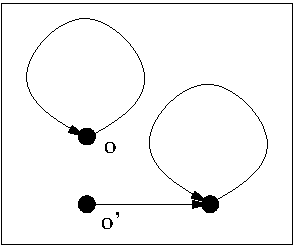
\includegraphics[scale=.8]{pic.pdf}
\end{center}
\caption{Distinguishable/indistinguishable points.}\label{fig-car1}
\end{figure}
%
The individuals $i$ and $i'$ can easily be distinguished in first-order logic:
the formula $R(x,x)$ is true of $i$ and false in $i'$. The corresponding
referring expression for $i$ would be ``an individual relating to itself''.
But if we can only use propositional and relational information (equivalently, our grammar does not contain the word ``itself'') then $i$ and $i'$ are indistinguishable. Both
are ``individuals which are related to individuals which are related to individuals\ldots''

In what follows we will introduce two logical languages (called \el and \alc, see~\cite{baad:desc03}) which can naturally be mapped to standard grammatically correct expressions.  \el allows
for conjunctions of atomic and existentially quantified relational expressions (e.g.,
``a red book on a table'') while \alc is the extension of \el with full negation
(e.g., ``a book which is not red and is not on the floor'').

\begin{definition}
Formulas of $\alc$ are generated by the following grammar:
$$
\form ::= p \mid \neg \varphi \mid \varphi \sqcap \varphi' \mid \exists R. \varphi
$$
where $p$ is in the set of propositional symbols \prop, $R$ is in the set of relational symbols \rel, $\varphi$ and $\varphi'$ are in \form. $\el$ is the
negation-free fragment of $\alc$.

Formulas of both $\alc$ and $\el$ are interpreted in relational first-order models
$\gM = (\Delta^\gM,|\cdot|^\gM)$ where $W$ is an arbitrary non-empy set, and $|\cdot|^\gM$ is an interpretation
function such that:
$$
\begin{array}{ccl}
|p|^\gM & \subseteq & \Delta^\gM  \mbox{ for $p \in \prop$}\\
|R|^\gM & \subseteq & \Delta^\gM \times \Delta^\gM  \mbox{ for $R \in \rel$}\\
|\neg \varphi|^\gM & = & W \backslash |\varphi|^\gM\\
|\varphi \wedge \varphi'|^\gM & = & |\varphi|^\gM \cap |\varphi'|^\gM\\
|\exists R.\varphi|^\gM & = & \{i \mid \mbox{for some } i' ((i,i') \in |R|^\gM)\\
& & \mbox{ and } i' \in |\varphi|^\gM \}.\\
\end{array}
$$
Given a model $\gM$ and an individual $i$ in the domain of $\gM$, let
$\propm(i) = \{p \in \prop \mid i \in |p|^\gM\}$.
\end{definition}

We can now exactly characterize the problem of when a formula distinguishing two
individuals in a given model exists. We will do so using the notion of \emph{bisimulation}.

\begin{definition}
Given a model $\gM = (\Delta^\gM,|\cdot|^\gM)$, two elements $i$ and $i'$ of $\Delta^\gM$ are $\alc$-bisimilar if it is possible to find a relation $Z \subseteq \Delta^\gM \times \Delta^\gM$ such that
\begin{enumerate}
\item $(i,i') \in Z$.
\item if $(e_1, e_2) \in Z$ then $\propm(e_1) = \propm(e_2)$.
\item if $(e_1,e_2) \in Z$ and for some $R \in \rel$ there is $e_1'$ such that
$(e_1,e_1') \in |R|^\gM$ then there is $e_2'$ such that $(e_2,e_2') \in |R|^\gM$ and
$(e_1',e_2') \in Z$.
\item if $(e_1,e_2) \in Z$ and for some $R \in \rel$ there is $e_2'$ such that
$(e_2,e_2') \in |R|^\gM$ then there is $e_1'$ such that $(e_1,e_1') \in |R|^\gM$ and
$(e_1',e_2') \in Z$.
\end{enumerate}
\end{definition}

\begin{theorem}[\cite{blac:moda01}]\label{bisim}
Given a model $\gM$, if  $i$ and $i'$ are two $\alc$-bisimilar elements in $\gM$
then there is no $\alc$-formula $\varphi$ such that $i \in |\varphi|^\gM$ and
$i' \not \in |\varphi|^\gM$.
\end{theorem}

In other words, $\alc$-bisimilar elements are indistinguishable in the $\alc$ langauge.
If we only consider finite models (actually, it is enought if we consider models where each element has only a finite number of immediate successors) then the converse of Theorem~\ref{bisim} also holds.

\begin{theorem}[\cite{blac:moda01}]\label{bisim2}
Given a model $\gM$, $i$ and $i'$ are two $\alc$-bisimilar elements in $\gM$
if and only if there is no $\alc$-formula $\varphi$ such that $i \in |\varphi|^\gM$ and
$i' \not \in |\varphi|^\gM$.
\end{theorem}

By defining a suitable notion of $\el$-bisimulation, the same results can be proved for
the $\el$ language. 

\cite{paig:thre87}

\cite{dovier04:_effic_algor_for_comput_bisim_equiv}

%%% Local Variables: 
%%% mode: latex
%%% TeX-master: "dl-gre-08"
%%% End: 
